%% V1.0
%% by Ussama Naal, usa.naal@gmail.com
%% Trying to be Udacious!

\documentclass[10pt,journal,compsoc]{IEEEtran}

\usepackage[pdftex]{graphicx}    
\usepackage{cite}
\usepackage{fullpage}
\usepackage{times}
\usepackage{fancyhdr,graphicx,amsmath,amssymb}
\usepackage[ruled,vlined]{algorithm2e}
\usepackage{url}
\include{pythonlisting}
\hyphenation{op-tical net-works semi-conduc-tor}


\begin{document}

\title{World Mapping Using ROS RTAB-Map}

\author{Ussama Naal}

\markboth{Paricles Filter, Robotic Nanodegree, Udacity}%
{}
\IEEEtitleabstractindextext{%

\begin{abstract}
This work. investigates the use of one implementation of a Graph-based SLAM known as RTAB-Map, in order to create a 3D mapping of a given site. Within a simulated environment used Gazebo and ROS, we deploy a two wheeled robot equipped with a laser scanner and an RGB-D camera and runs a ros package that implements the RTAB-Map algorithm. We test the configured robot under two different sites and demonstrate obtained results.
\end{abstract}

% Note that keywords are not normally used for peer-review papers.
\begin{IEEEkeywords}
world mapping, ROS, slam, GraphSLAM, RTAB-Map.
\end{IEEEkeywords}}


\maketitle
\IEEEdisplaynontitleabstractindextext
\IEEEpeerreviewmaketitle
\section{Introduction}
\label{sec:introduction}

%TODO Real Time Appearance Based Mapping

\IEEEPARstart Successful robot navigation requires having an accurate representation of the world that robot traverses through. When a detailed map of the world is not readily available to the robot or current map is not up to date, in the case, the robot could rely on its sensors to survey the site and build a good approximation of the site. Moreover, since the set of the sensors that the robot rely on could be subject to noise and inaccuracies which leads to drift in the robot position, the robot can at the same time utilize the map being created in order to find the actual location of the robot within the map. This process is known as Simultaneous Localization and Mapping (SLAM). In next section we outline the problem and available solutions. In section 3, we review our robot configuration. In section 4, we review achieved results when running the RTAB-Map algorithm against two different environments. We discuss these results in section 5. Finally, in section 6, we provide conclusions and hint at future work.

\section{Background / Formulation}


SLAM deals with the case when the robot has only access to its sensors data and knowledge of its own movement. Using available data the robots tries to estimate the map and its position within the estimated map. The main challenge with estimating the map lies within the count of state variable to describe the map. Another challenge is when dealing with a representation that contain repetitive patterns causing uncertainty when estimating the robot pose. Known SLAM-based approaches can be categorized into five categories: Extended Kalman Filter SLAM (EKF) \cite{ekf-slam-wiki}, Sparse Extended Filter Information SLAM (SEIF) \cite{seif}, Extended Information Form (EIF) \cite{maybeck1982stochastic}, FastSLAM \cite{Montemerlo02fastslam:a} and GraphSLAM \cite{thrun2006graph}.

In this work we employ the RTAB-Map which is GraphSLAM-based approach. In GraphSLAM, a graph is constructed where nodes represent estimated robot poses and estimated locations of landmarks or identifiable features on the map at a given point in time. Edges on the other hand represent constraints that connect between robot poses and the detected features on the map. There two types of constraints: motion constraint and measurement constraint. Motion constraints represent the distance between robot poses at different times, while measurement constraints represent the distance between a given pose and the distance to a nearby landmark of feature measured by the robot at that pose. Following figure shows this relationship.

\begin{figure}[thpb]
      \centering
      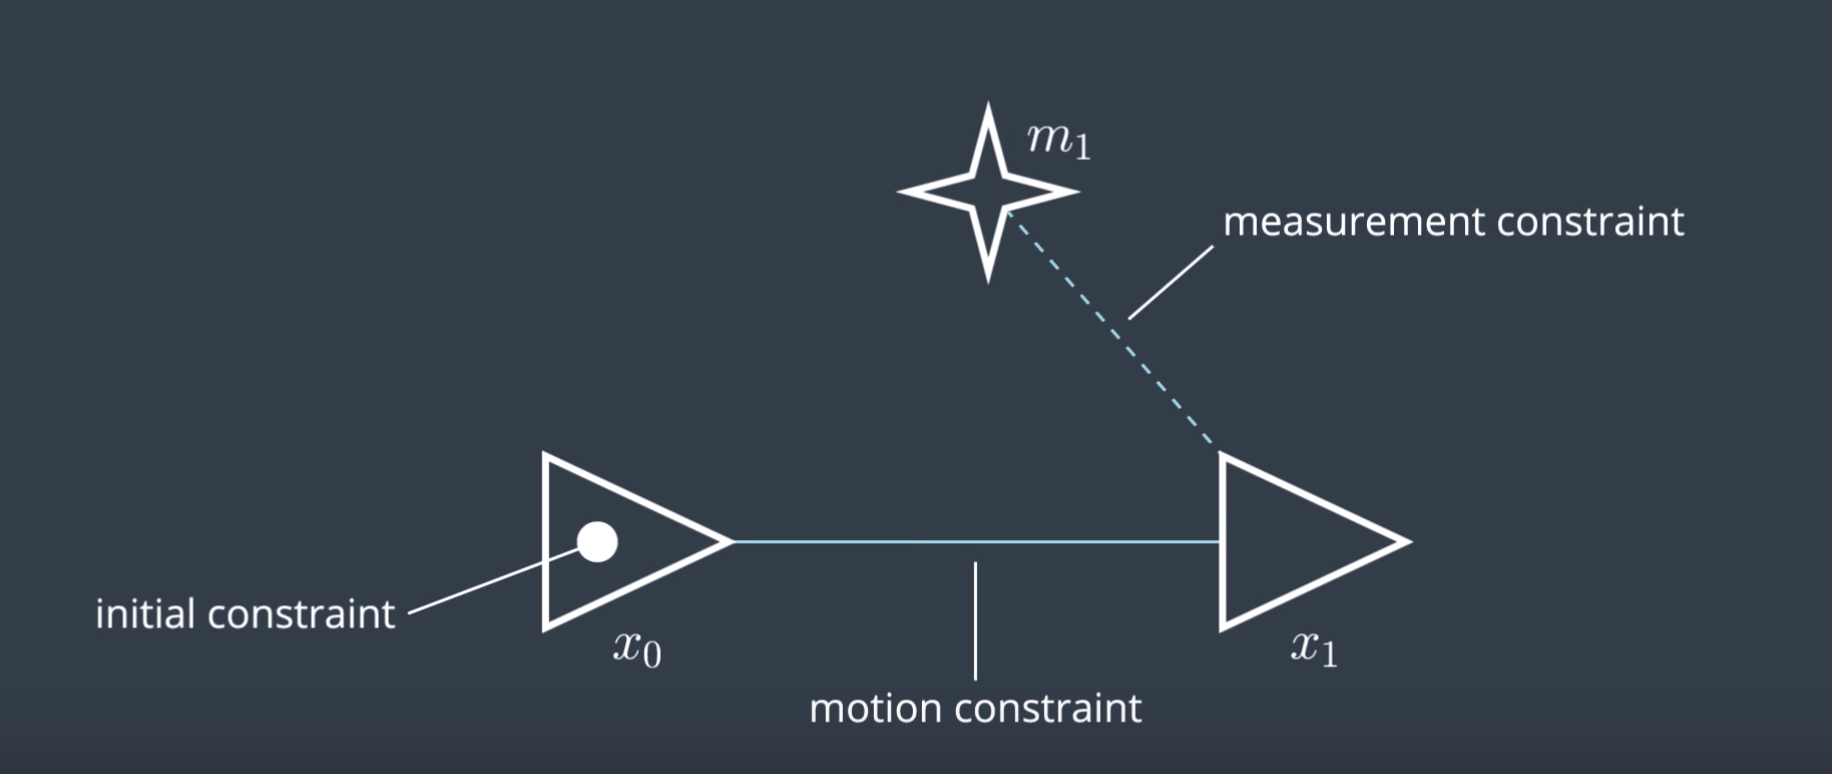
\includegraphics[width=\linewidth]{graph.png}
      \caption{Constraints Graph.}
      \label{fig:graph-slam}
\end{figure}

The robot continues to build the graph as it moves and survey its environment adding new nodes and constraints, however, due to noise and inaccuracies of estimated poses and measurements the constraints may not map properly. This results in an over-determined system which converts the problem into an optimization problem. To solve the system, graph data is organized into an information matrix and an information vector where cells represent the linearized constraint around an estimate between two given nodes. Both data structures gets passed to a numerical solver that returns most probable configuration of the graph.

In GraphSLAM it is essential to detect loop closures when surveying the environment, i.e. identify if the robot has observed the same place again. Detecting loop closures requires comparing current acquired scan of the environment against all previous scans.  This is a very daunting task since complexity increases linearly as the robot acquires new scans. The RTAB-Map performs a set of techniques to the original GraphSLAM to keep the process running near real-time. These techniques can be summarized in: Local/Global Loop Closure Detection, Visual Bag-of-Words, Memory Management.

\section{Robot Configuration}
We used the robot configuration used in the previous project \cite{ros-amcl-robot-navigation} with one exception. In this robot we replace previous RGB camera with a depth camera also known as an RGB-D camera.

\begin{figure}[thpb]
      \centering
      \includegraphics[width=\linewidth]{robot-in-kitchen.png}
      \caption{Robot in the kitchen environment.}
      \label{fig:network-training}
\end{figure}

We make sure to update the gazebo files such that sensors data are published to the channels.

\begin{figure}[thpb]
      \centering
      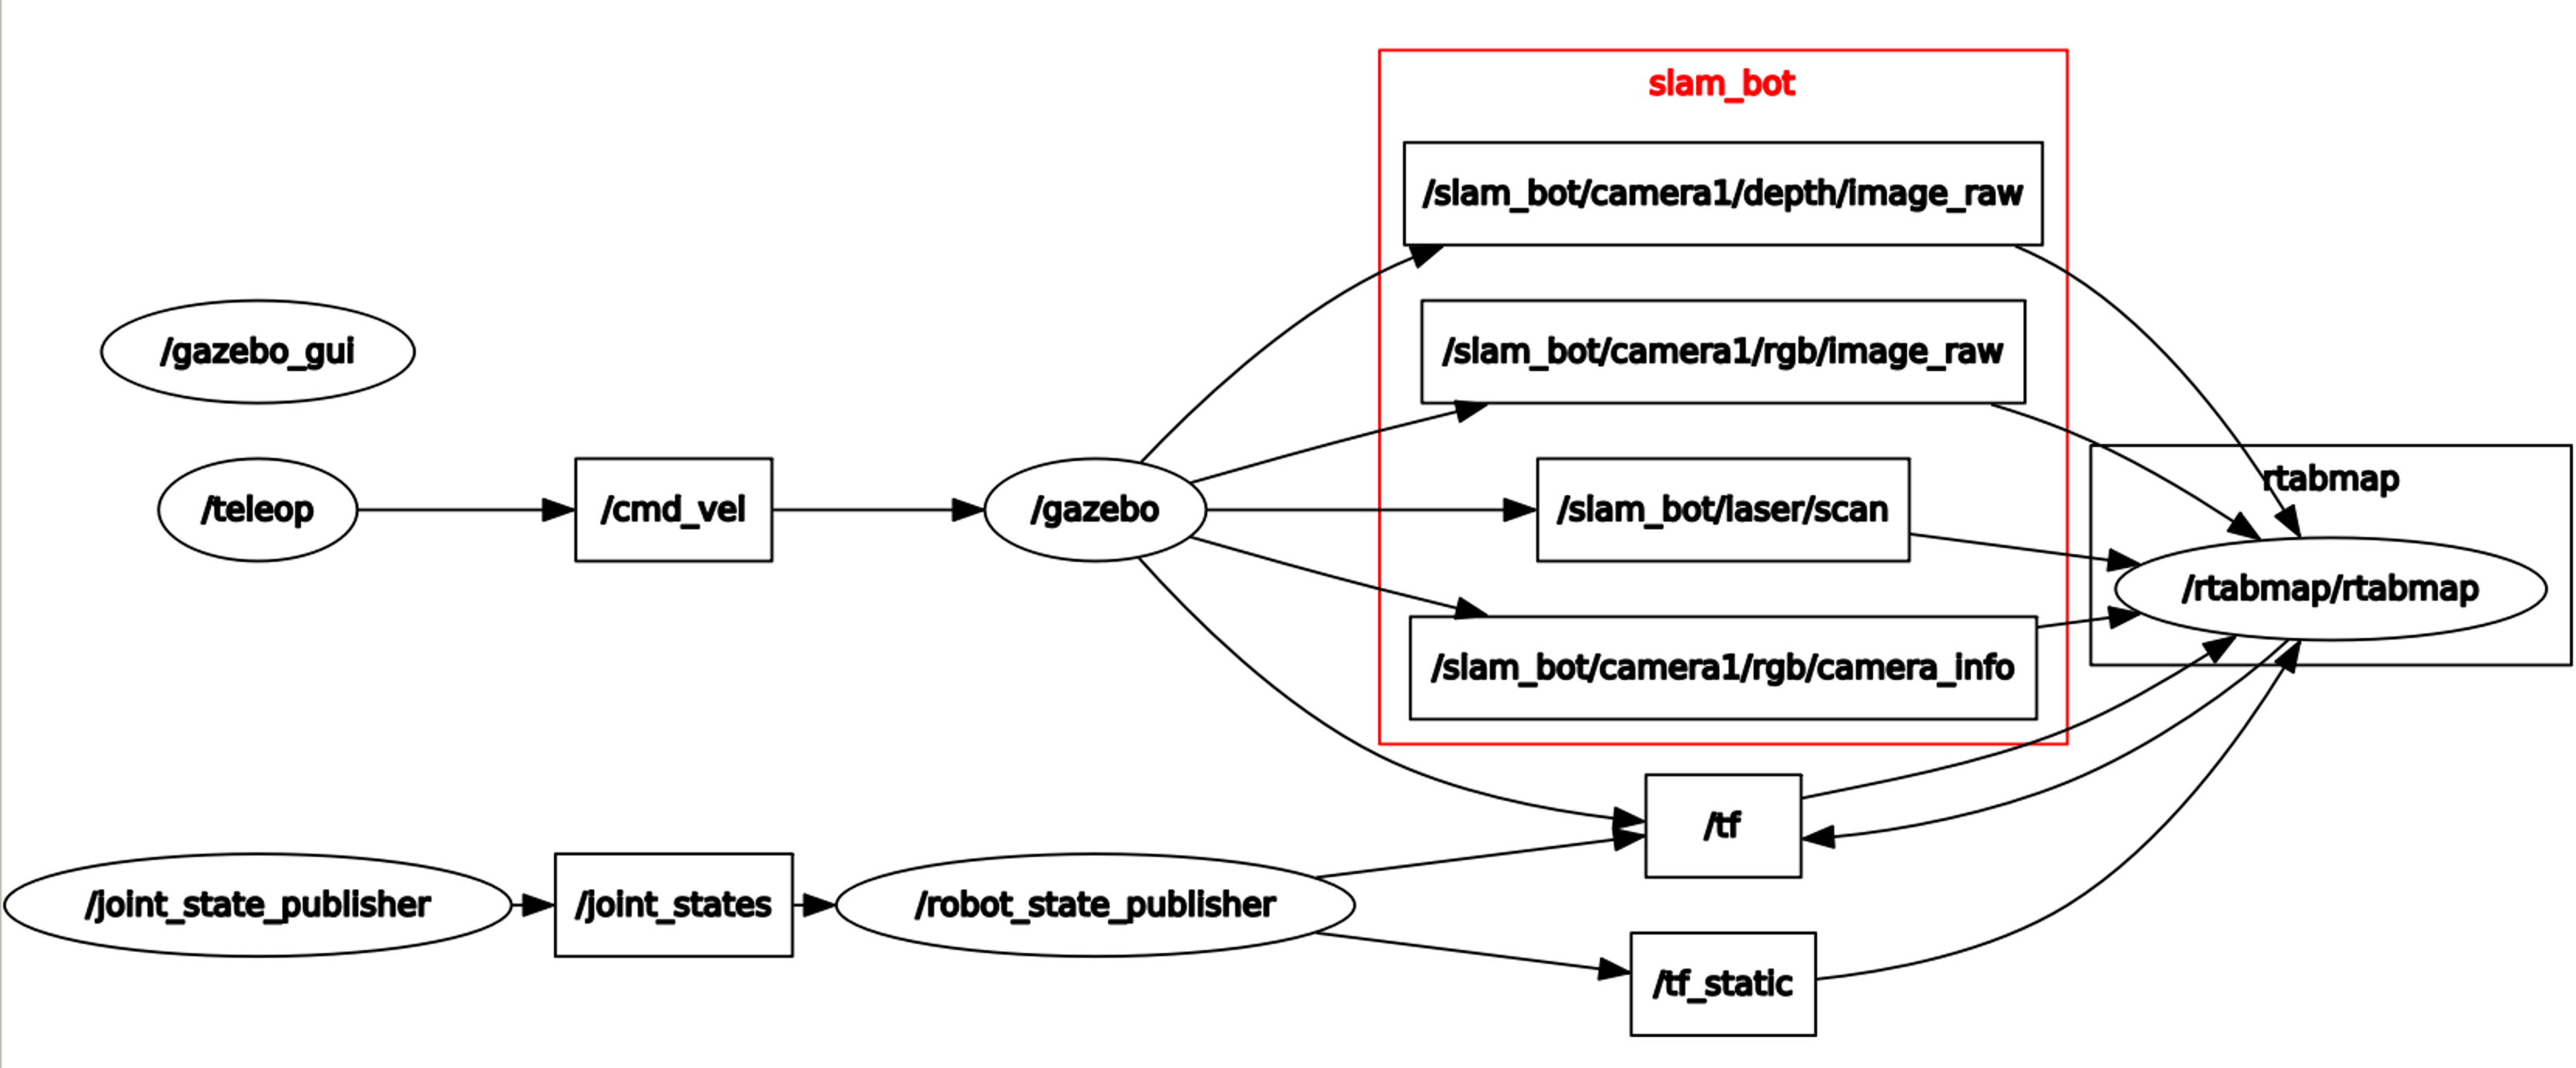
\includegraphics[width=\linewidth]{robot-graph.png}
      \caption{Robot Graph.}
      \label{fig:network-training}
\end{figure}

\section{Results}

In this section we review results obtained by deploying the robot with the same algorithm and configuration to two different environments. First environment is the kitchen environment and then a personal one.

\subsection{Kitchen Environment}

The following image shows the configuration of this environment within the simulator:

\begin{figure}[thpb]
      \centering
      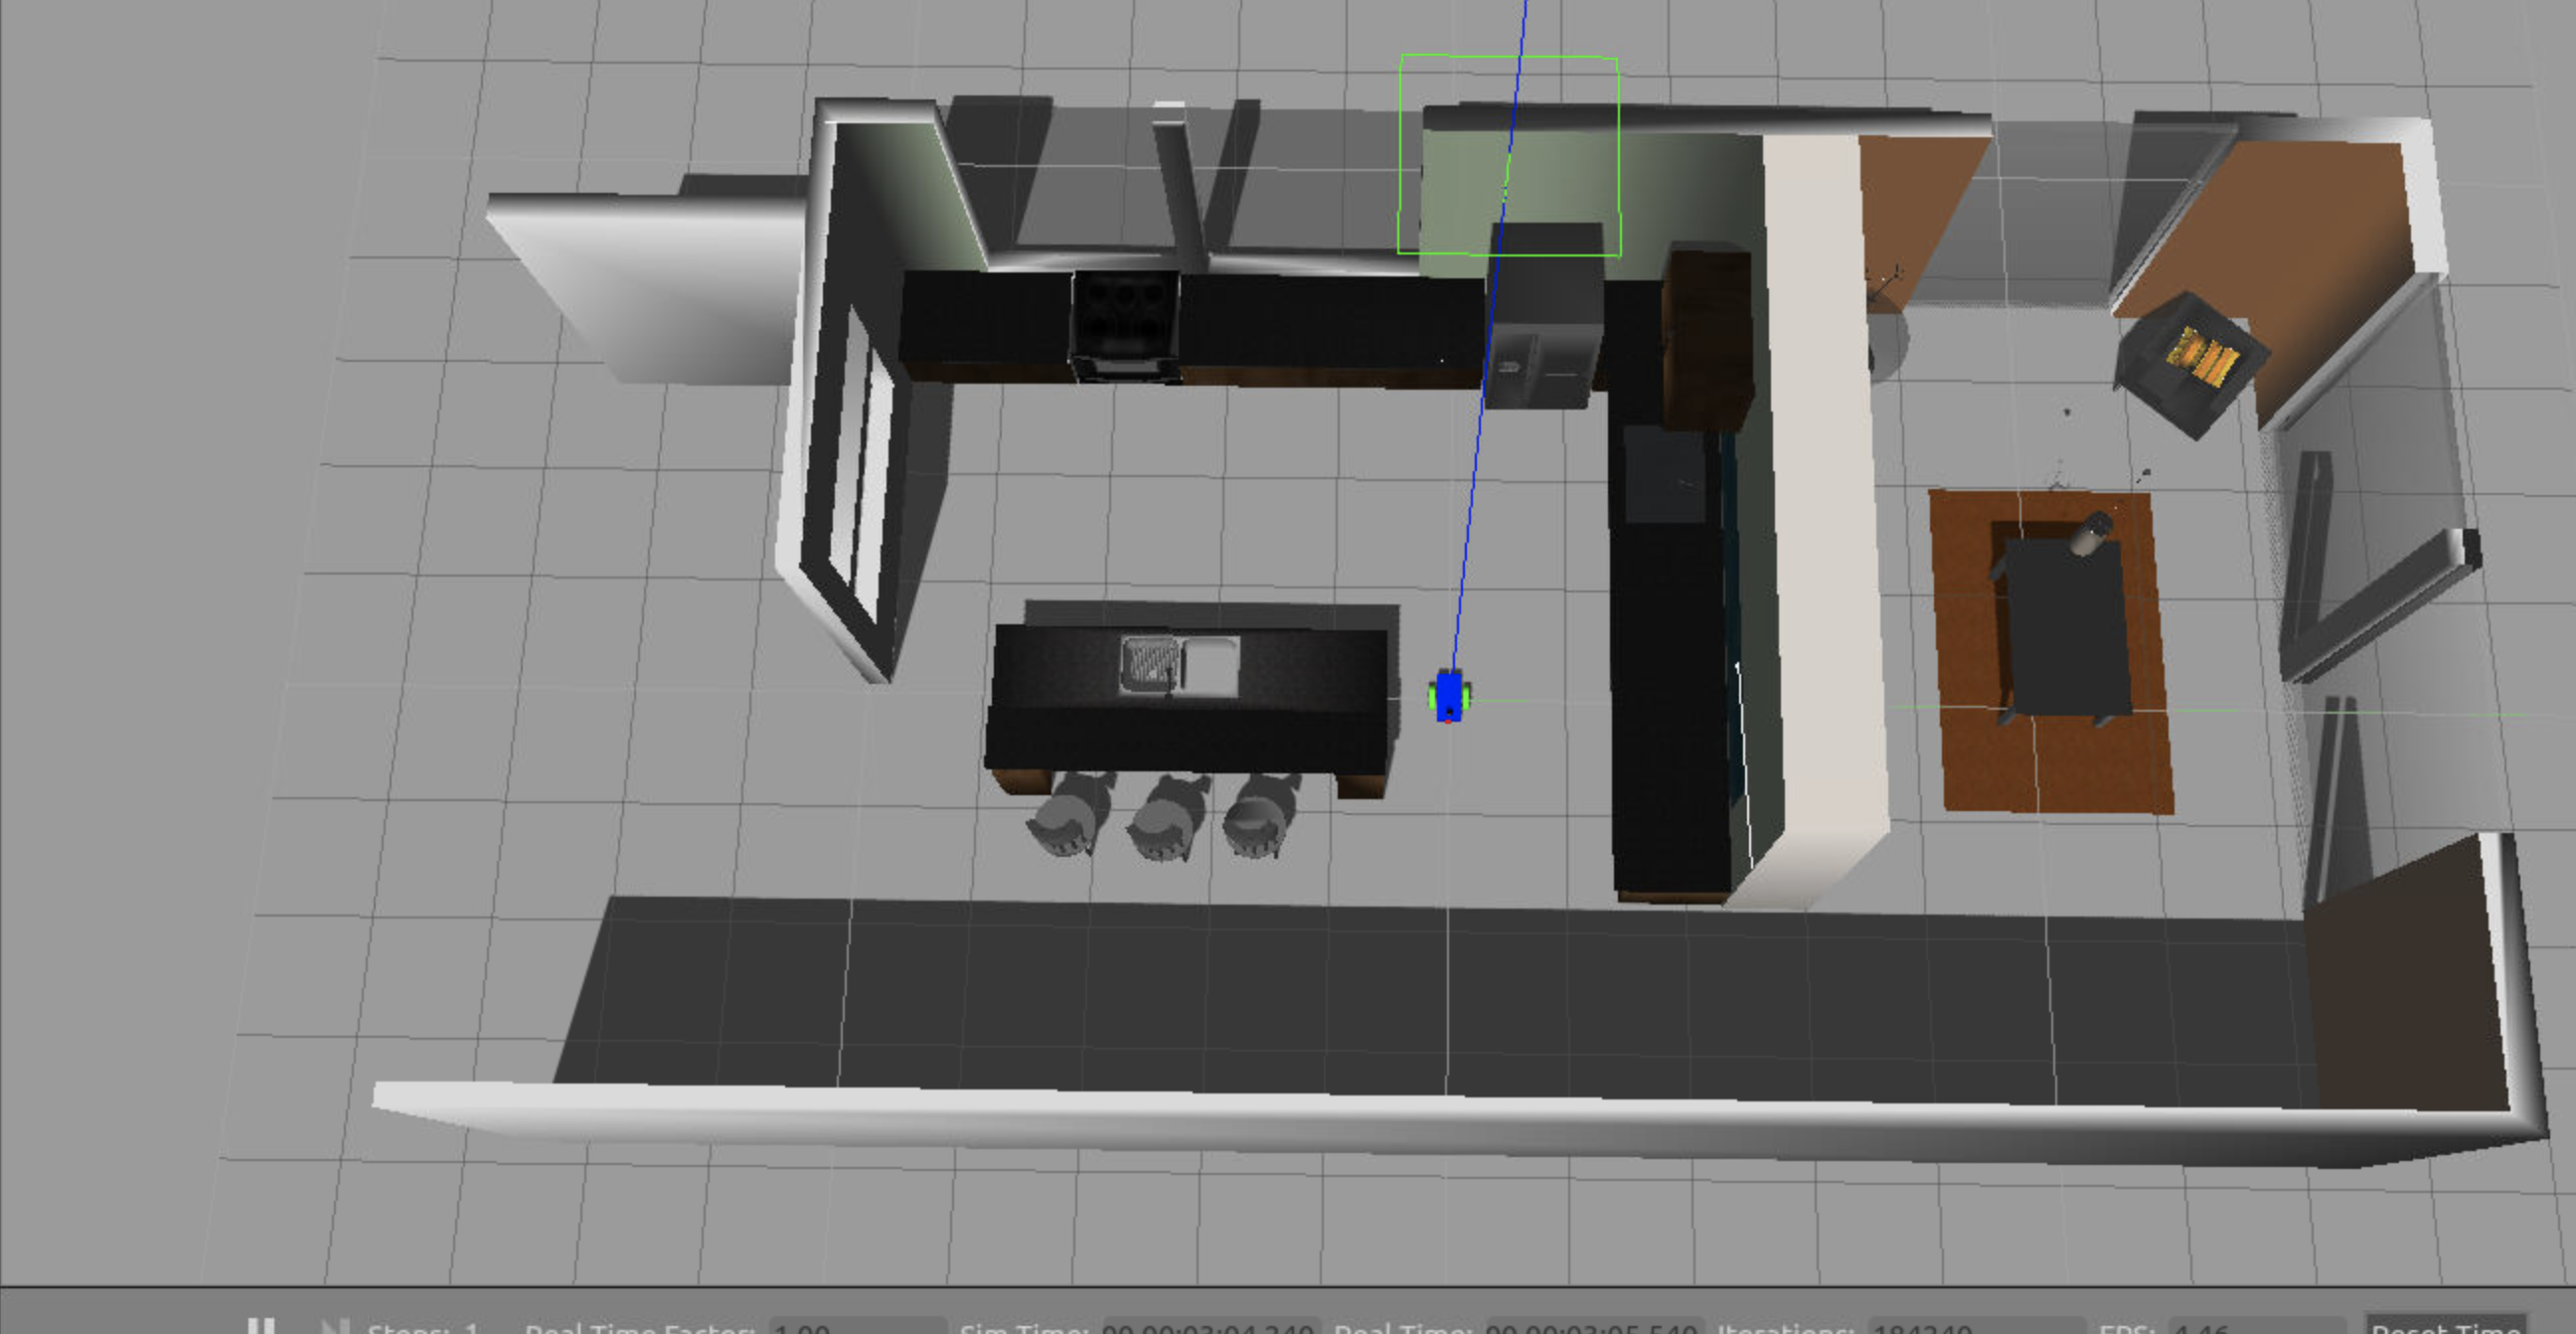
\includegraphics[width=\linewidth]{kitchen-environment.png}
      \caption{Kitchen Environment.}
      \label{fig:network-training}
\end{figure}

Images in figure 5 and 6 show the path took by the robot and the detected features and how these features where used to correspondence between two different frames.

\begin{figure}[thpb]
      \centering
      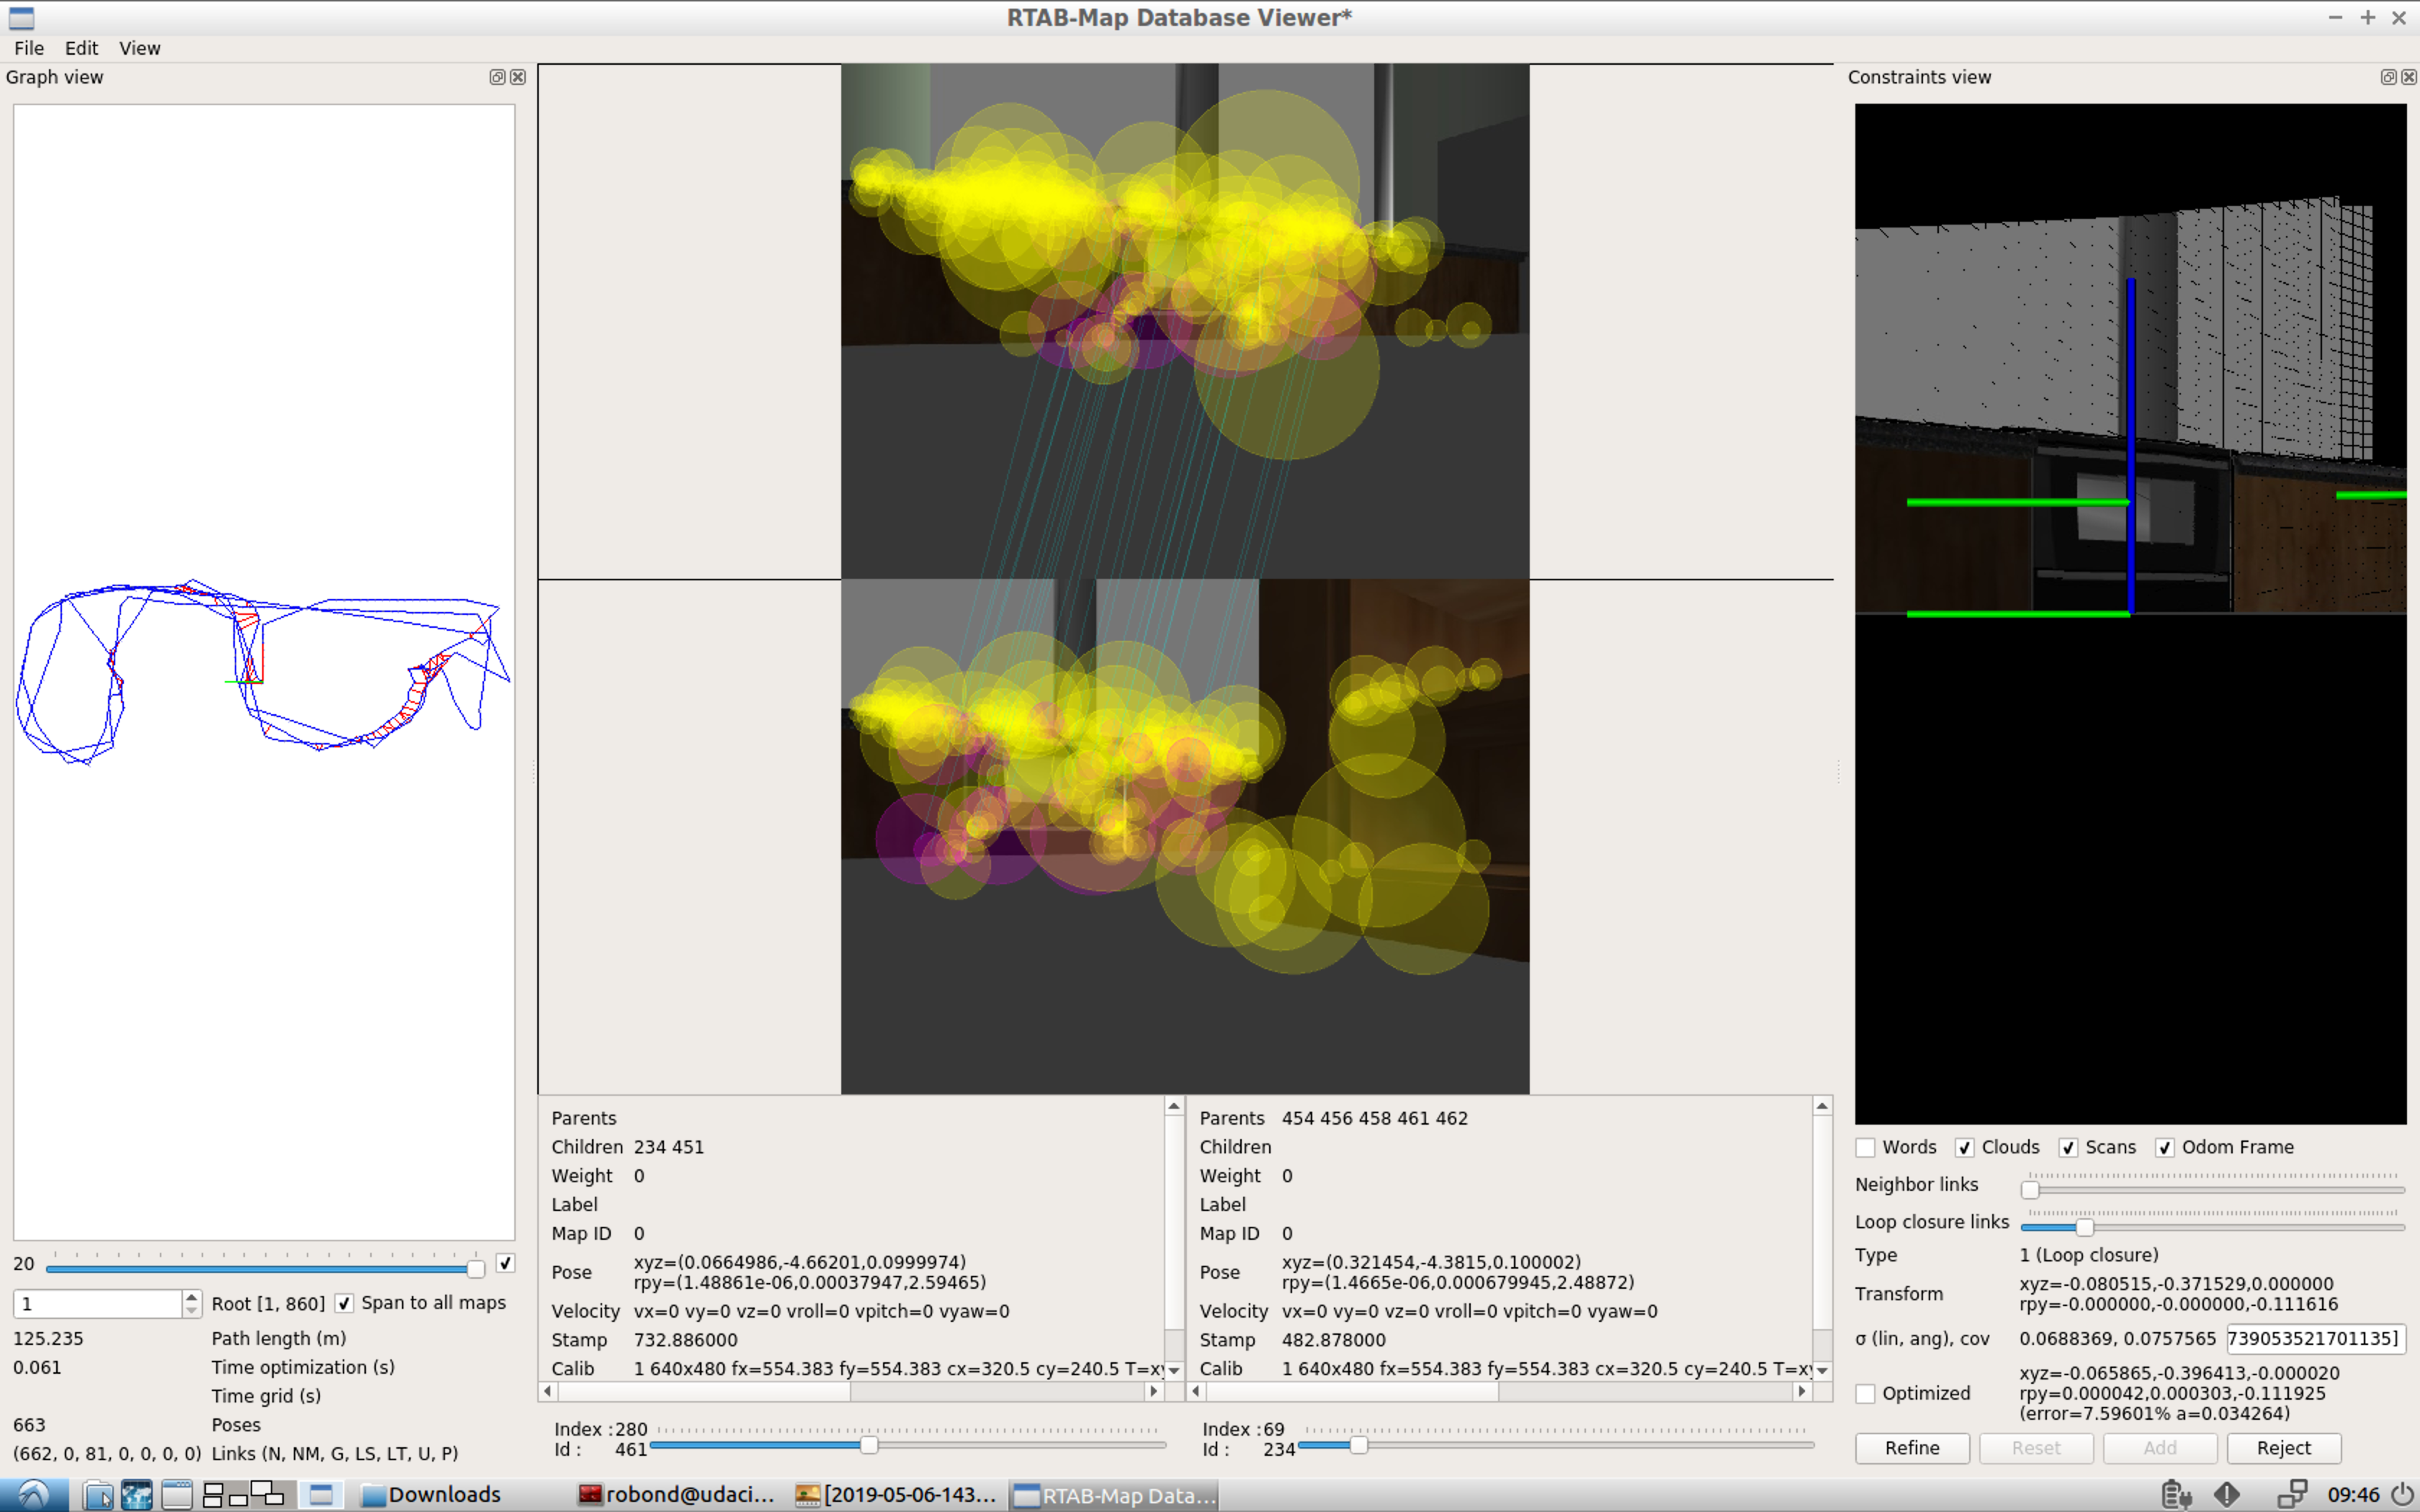
\includegraphics[width=\linewidth]{rtab-map-viewer.png}
      \caption{Kitchen Environment: Graph View and Feature Correspondence 1.}
      \label{fig:network-training}
\end{figure}

\begin{figure}[thpb]
      \centering
      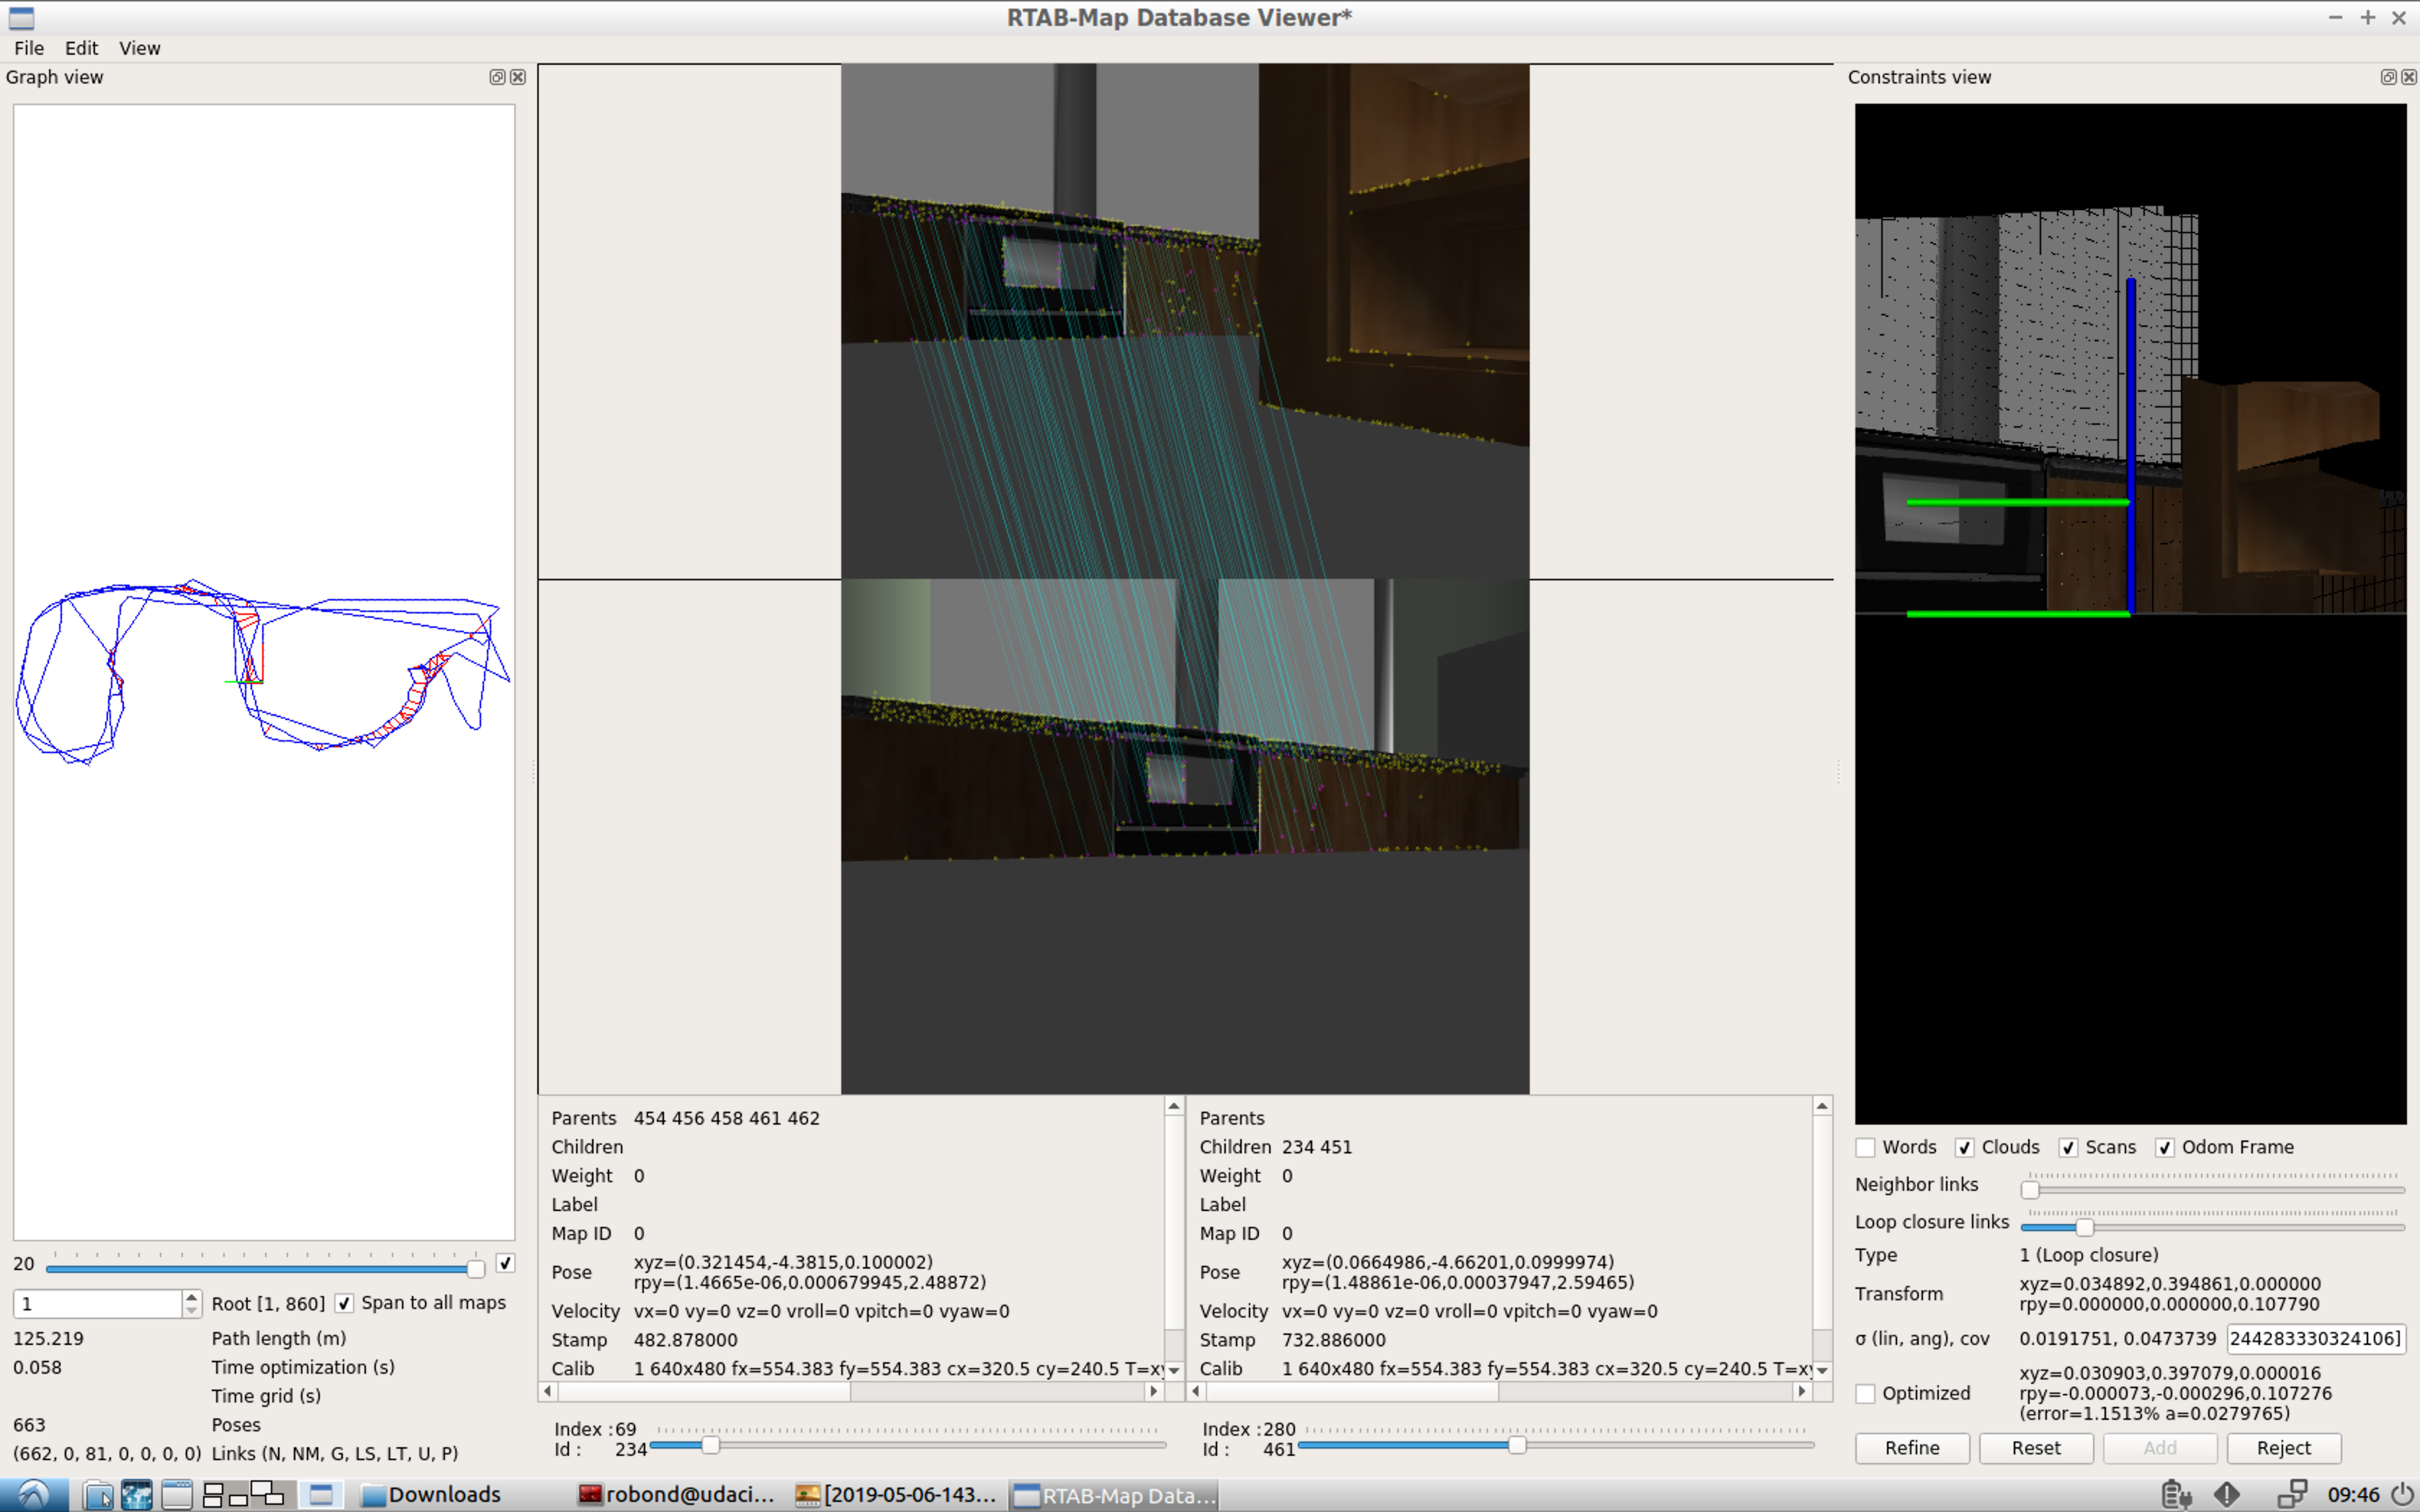
\includegraphics[width=\linewidth]{rtab-map-viewer-corresponence.png}
      \caption{Kitchen Environment: Graph View and Feature Correspondence 2.}
      \label{fig:network-training}
\end{figure}

Finally, Figure 7 shows 3D reconstructed point cloud of the kitchen environment. We can clearly see that RTAB-Map creates a good representation of the environment.

\begin{figure}[thpb]
      \centering
      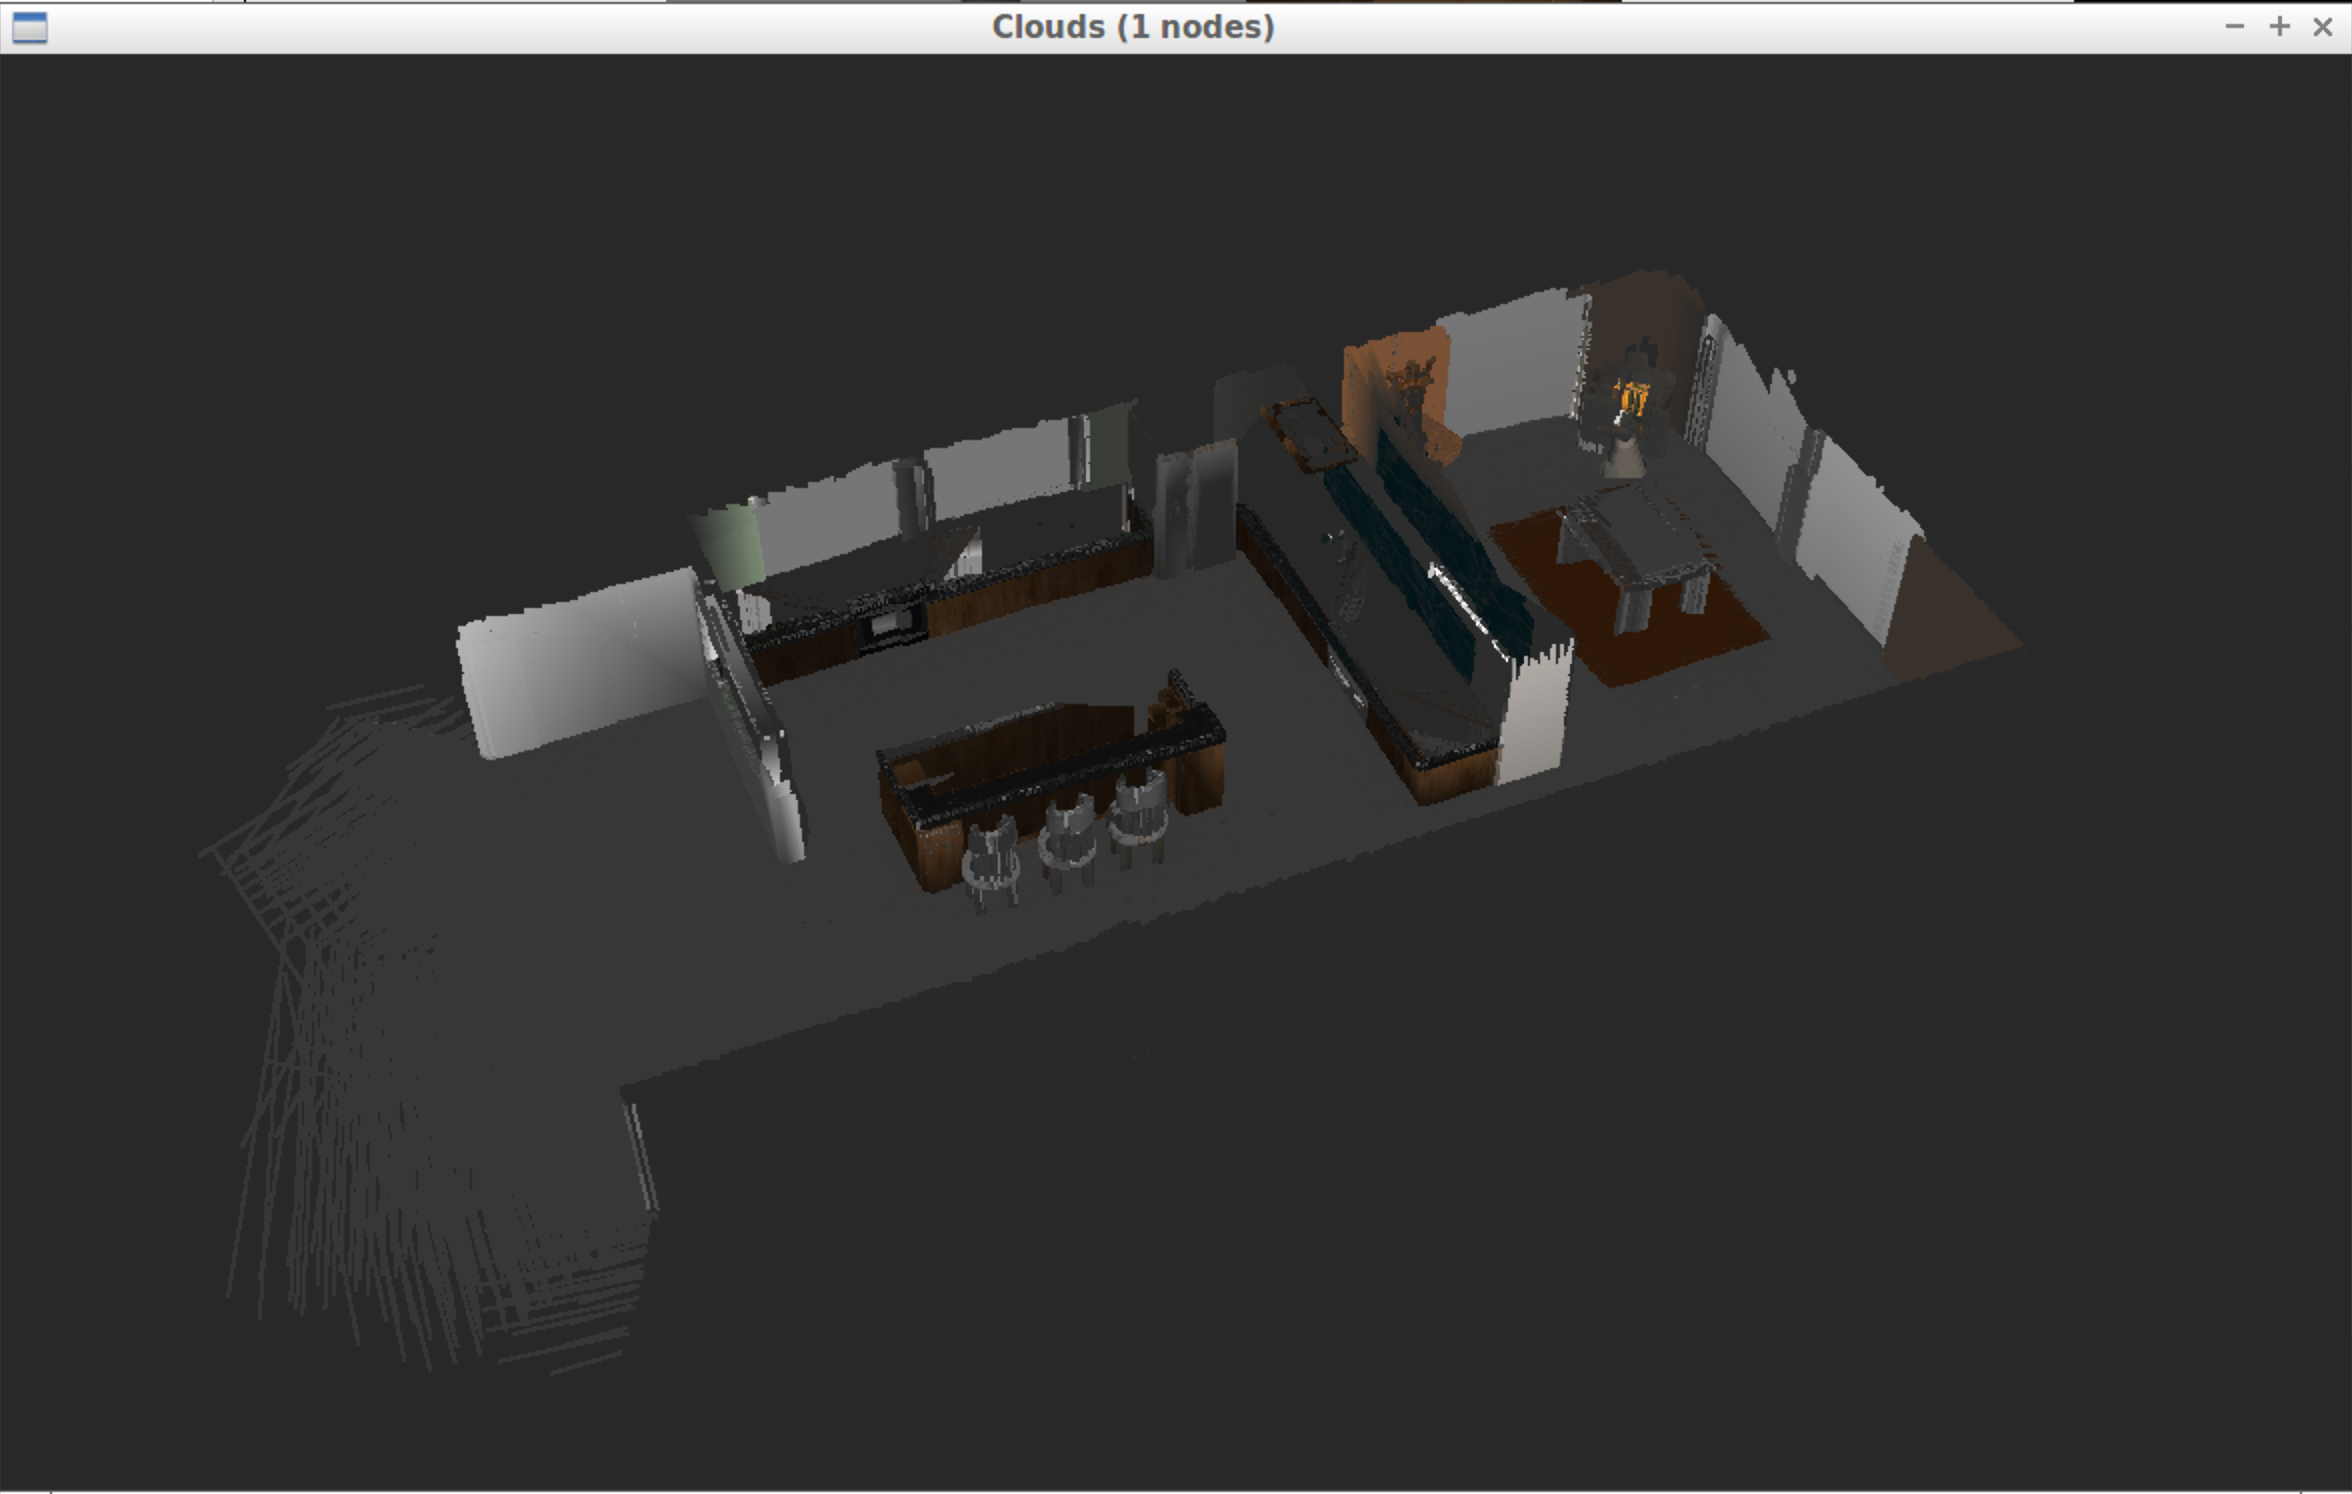
\includegraphics[width=\linewidth]{kitchen-point-cloud.png}
      \caption{Kitchen Environment: Point cloud generated through RTAB-Map.}
      \label{fig:network-training}
\end{figure}

\subsection{Personal Environment}

Using available objects in Gazebo, we construct personal environment that simulate site that has many wrecks and ambulance vehicle and few other objects and trees. Figure 8, displays the configuration used in the personal environment within the simulator.

\begin{figure}[thpb]
      \centering
      \includegraphics[width=\linewidth]{personal-environment.png}
      \caption{Personal Environment.}
      \label{fig:network-training}
\end{figure}

Same in previous sub-section, We show the two following images show the path took by the robot and the detected features and how these features where used to correspondence between two different frames:

\begin{figure}[thpb]
      \centering
      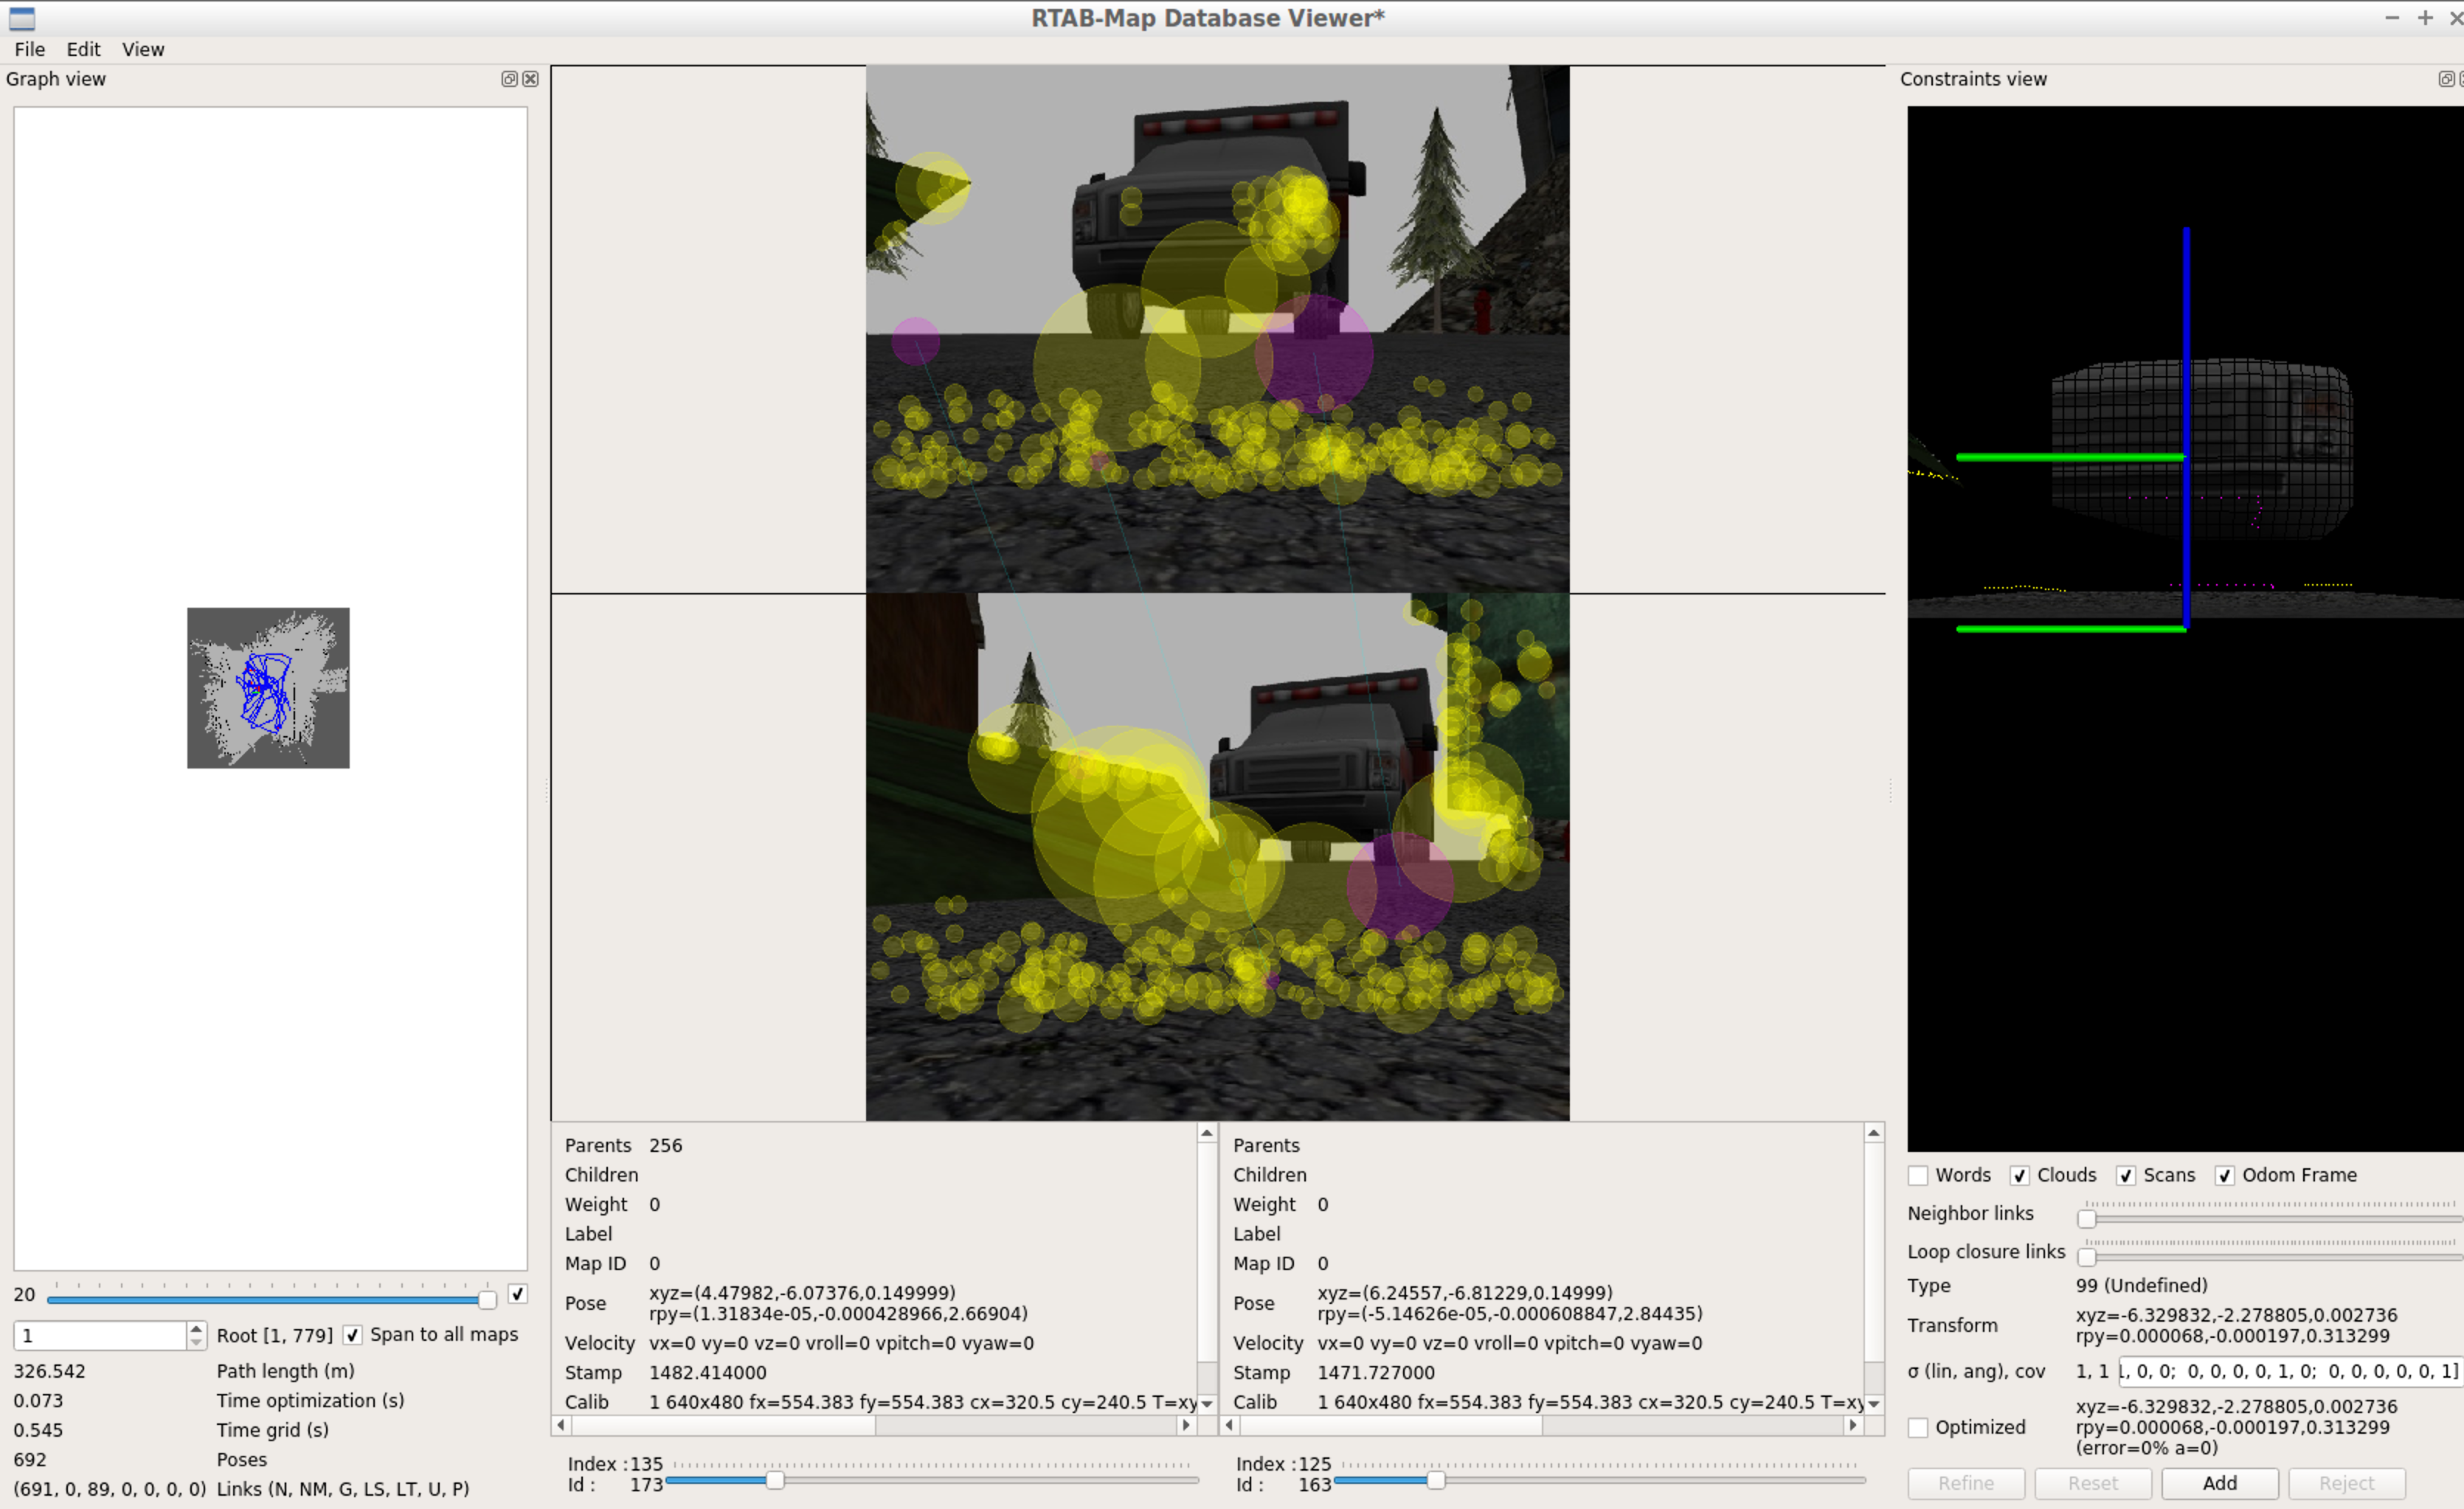
\includegraphics[width=\linewidth]{rtab-map-viewer-correspondence1.png}
      \caption{Personal Environment: Graph View and Feature Correspondence 1.}
      \label{fig:network-training}
\end{figure}

\begin{figure}[thpb]
      \centering
      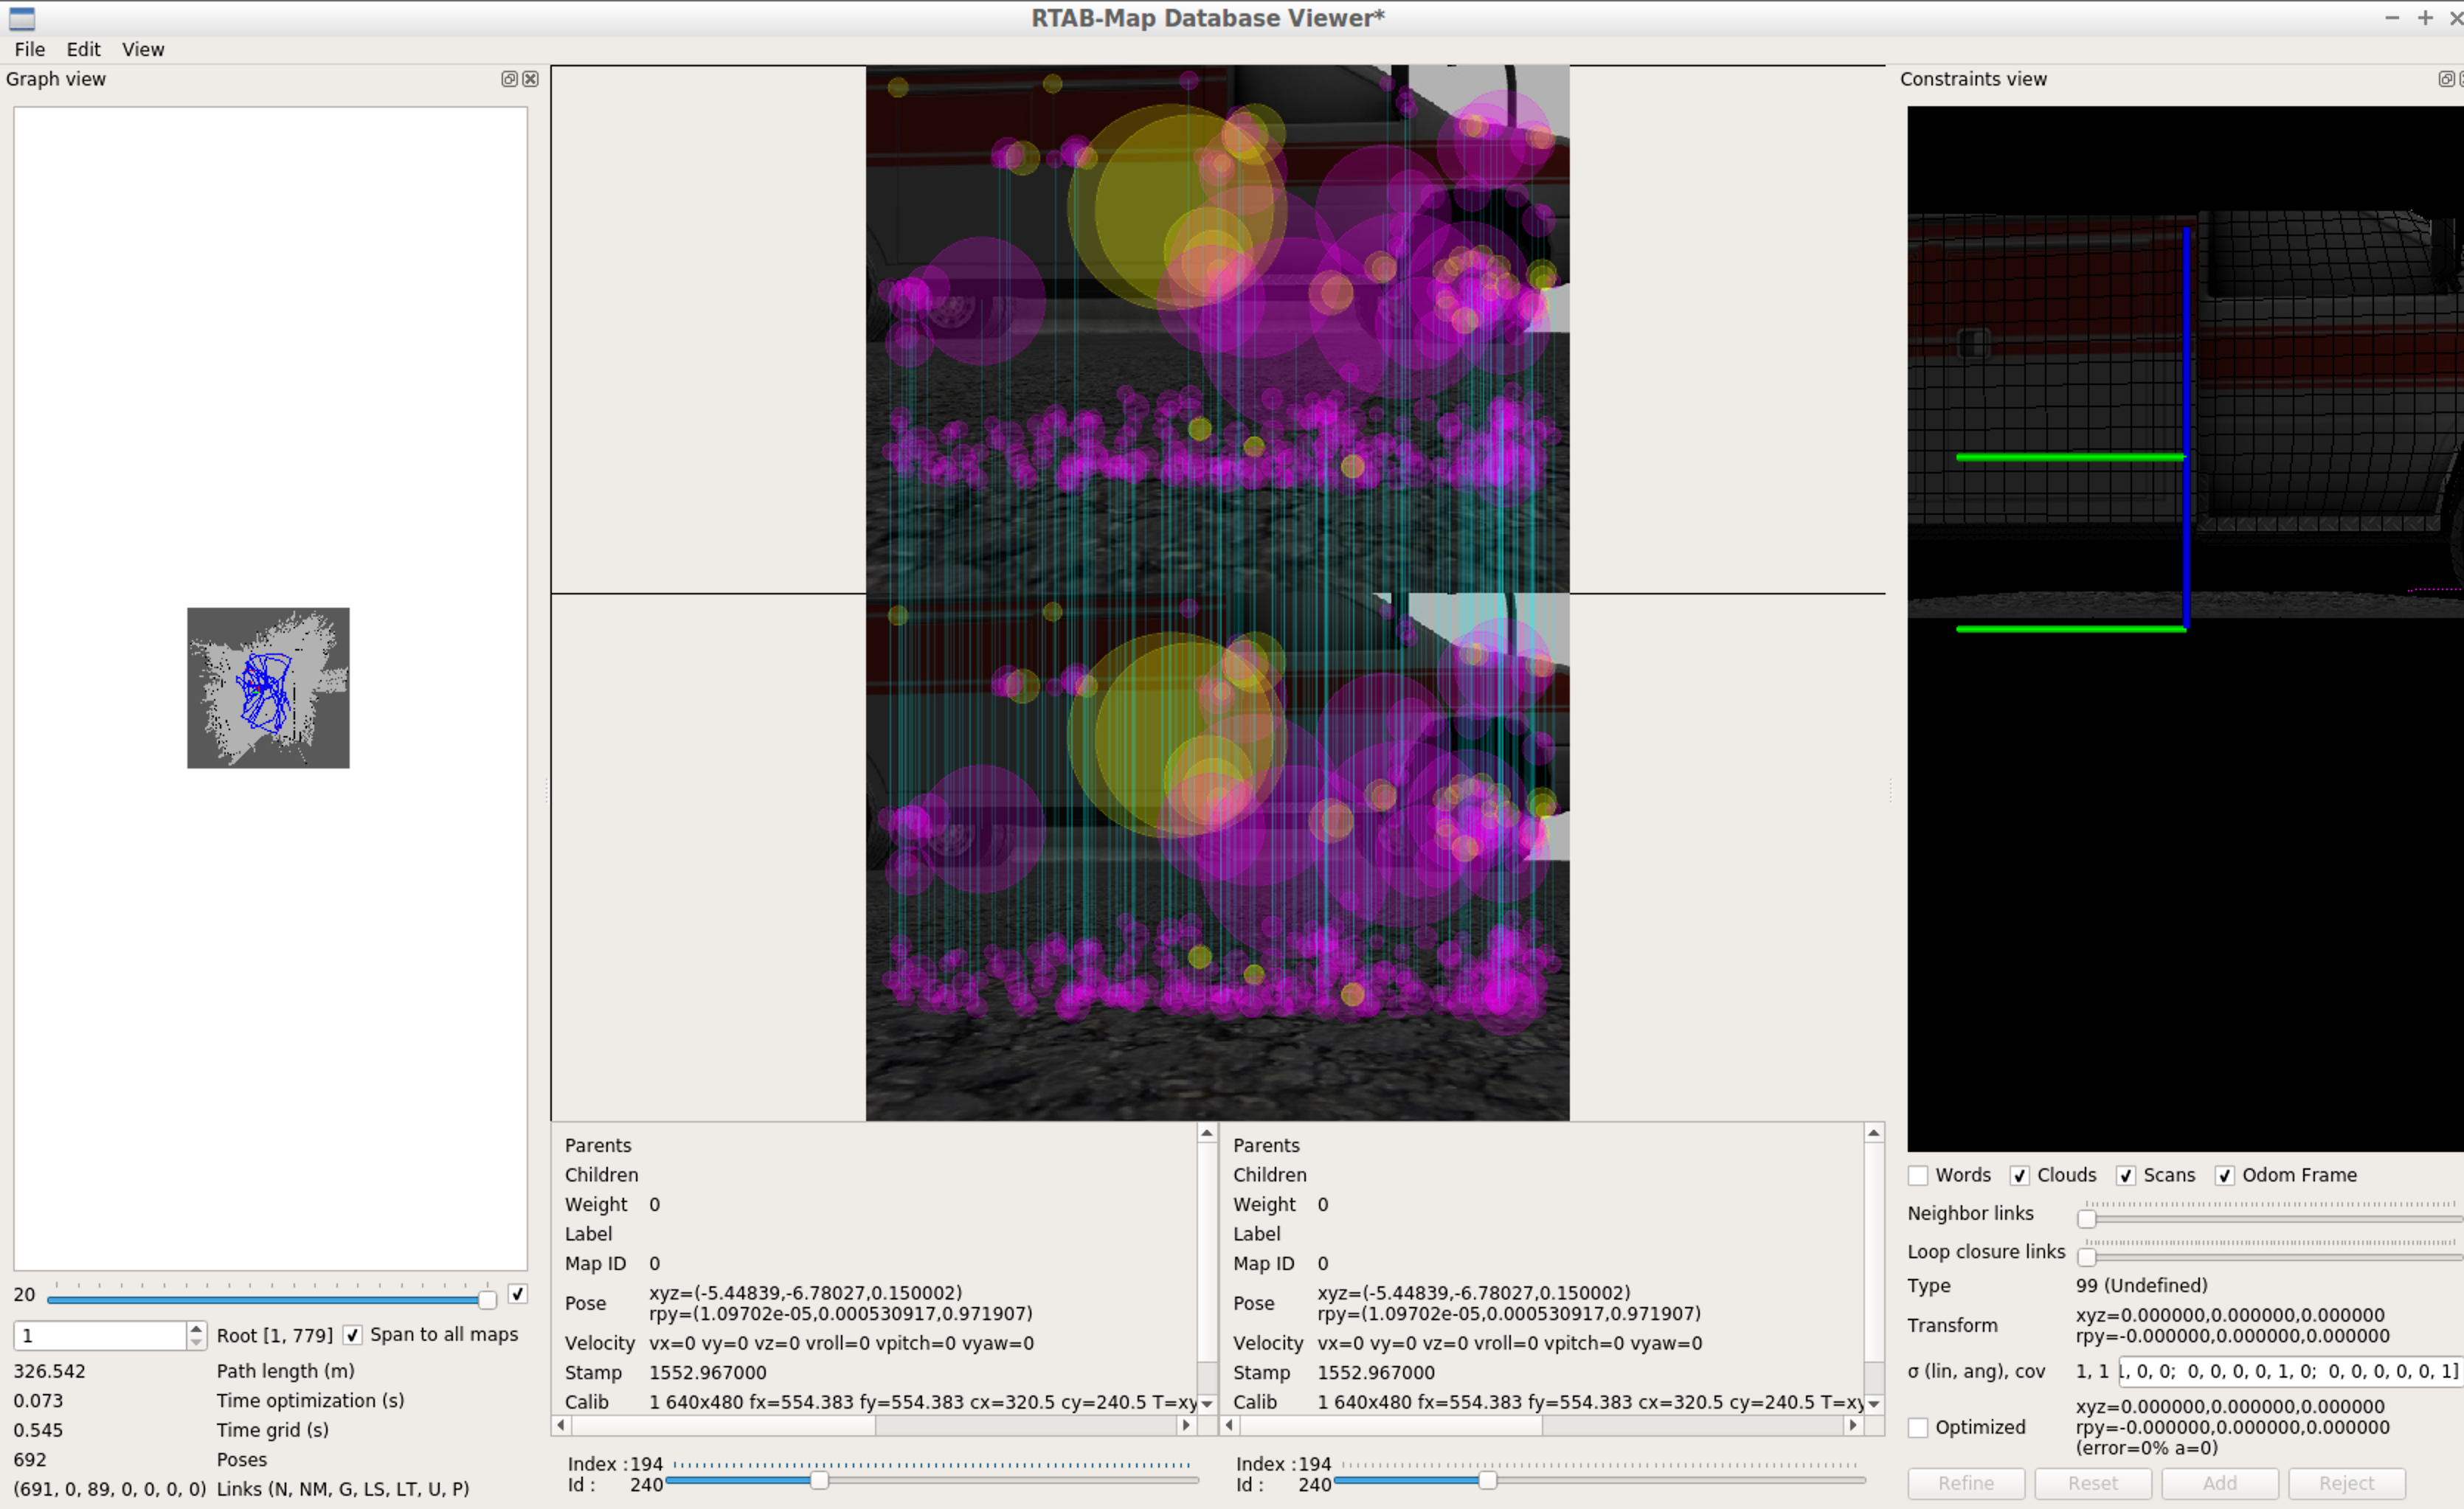
\includegraphics[width=\linewidth]{rtab-map-viewer-correspondence2.png}
      \caption{Personal Environment: Graph View and Feature Correspondence 2.}
      \label{fig:network-training}
\end{figure}

Lastly, next image shows 3D reconstructed point cloud of the personal environment. We can observe partial re-construction of the scene but the algorithm was successful at closing loops, which caused discontinuities for the 3D constructed scene.

\begin{figure}[thpb]
      \centering
      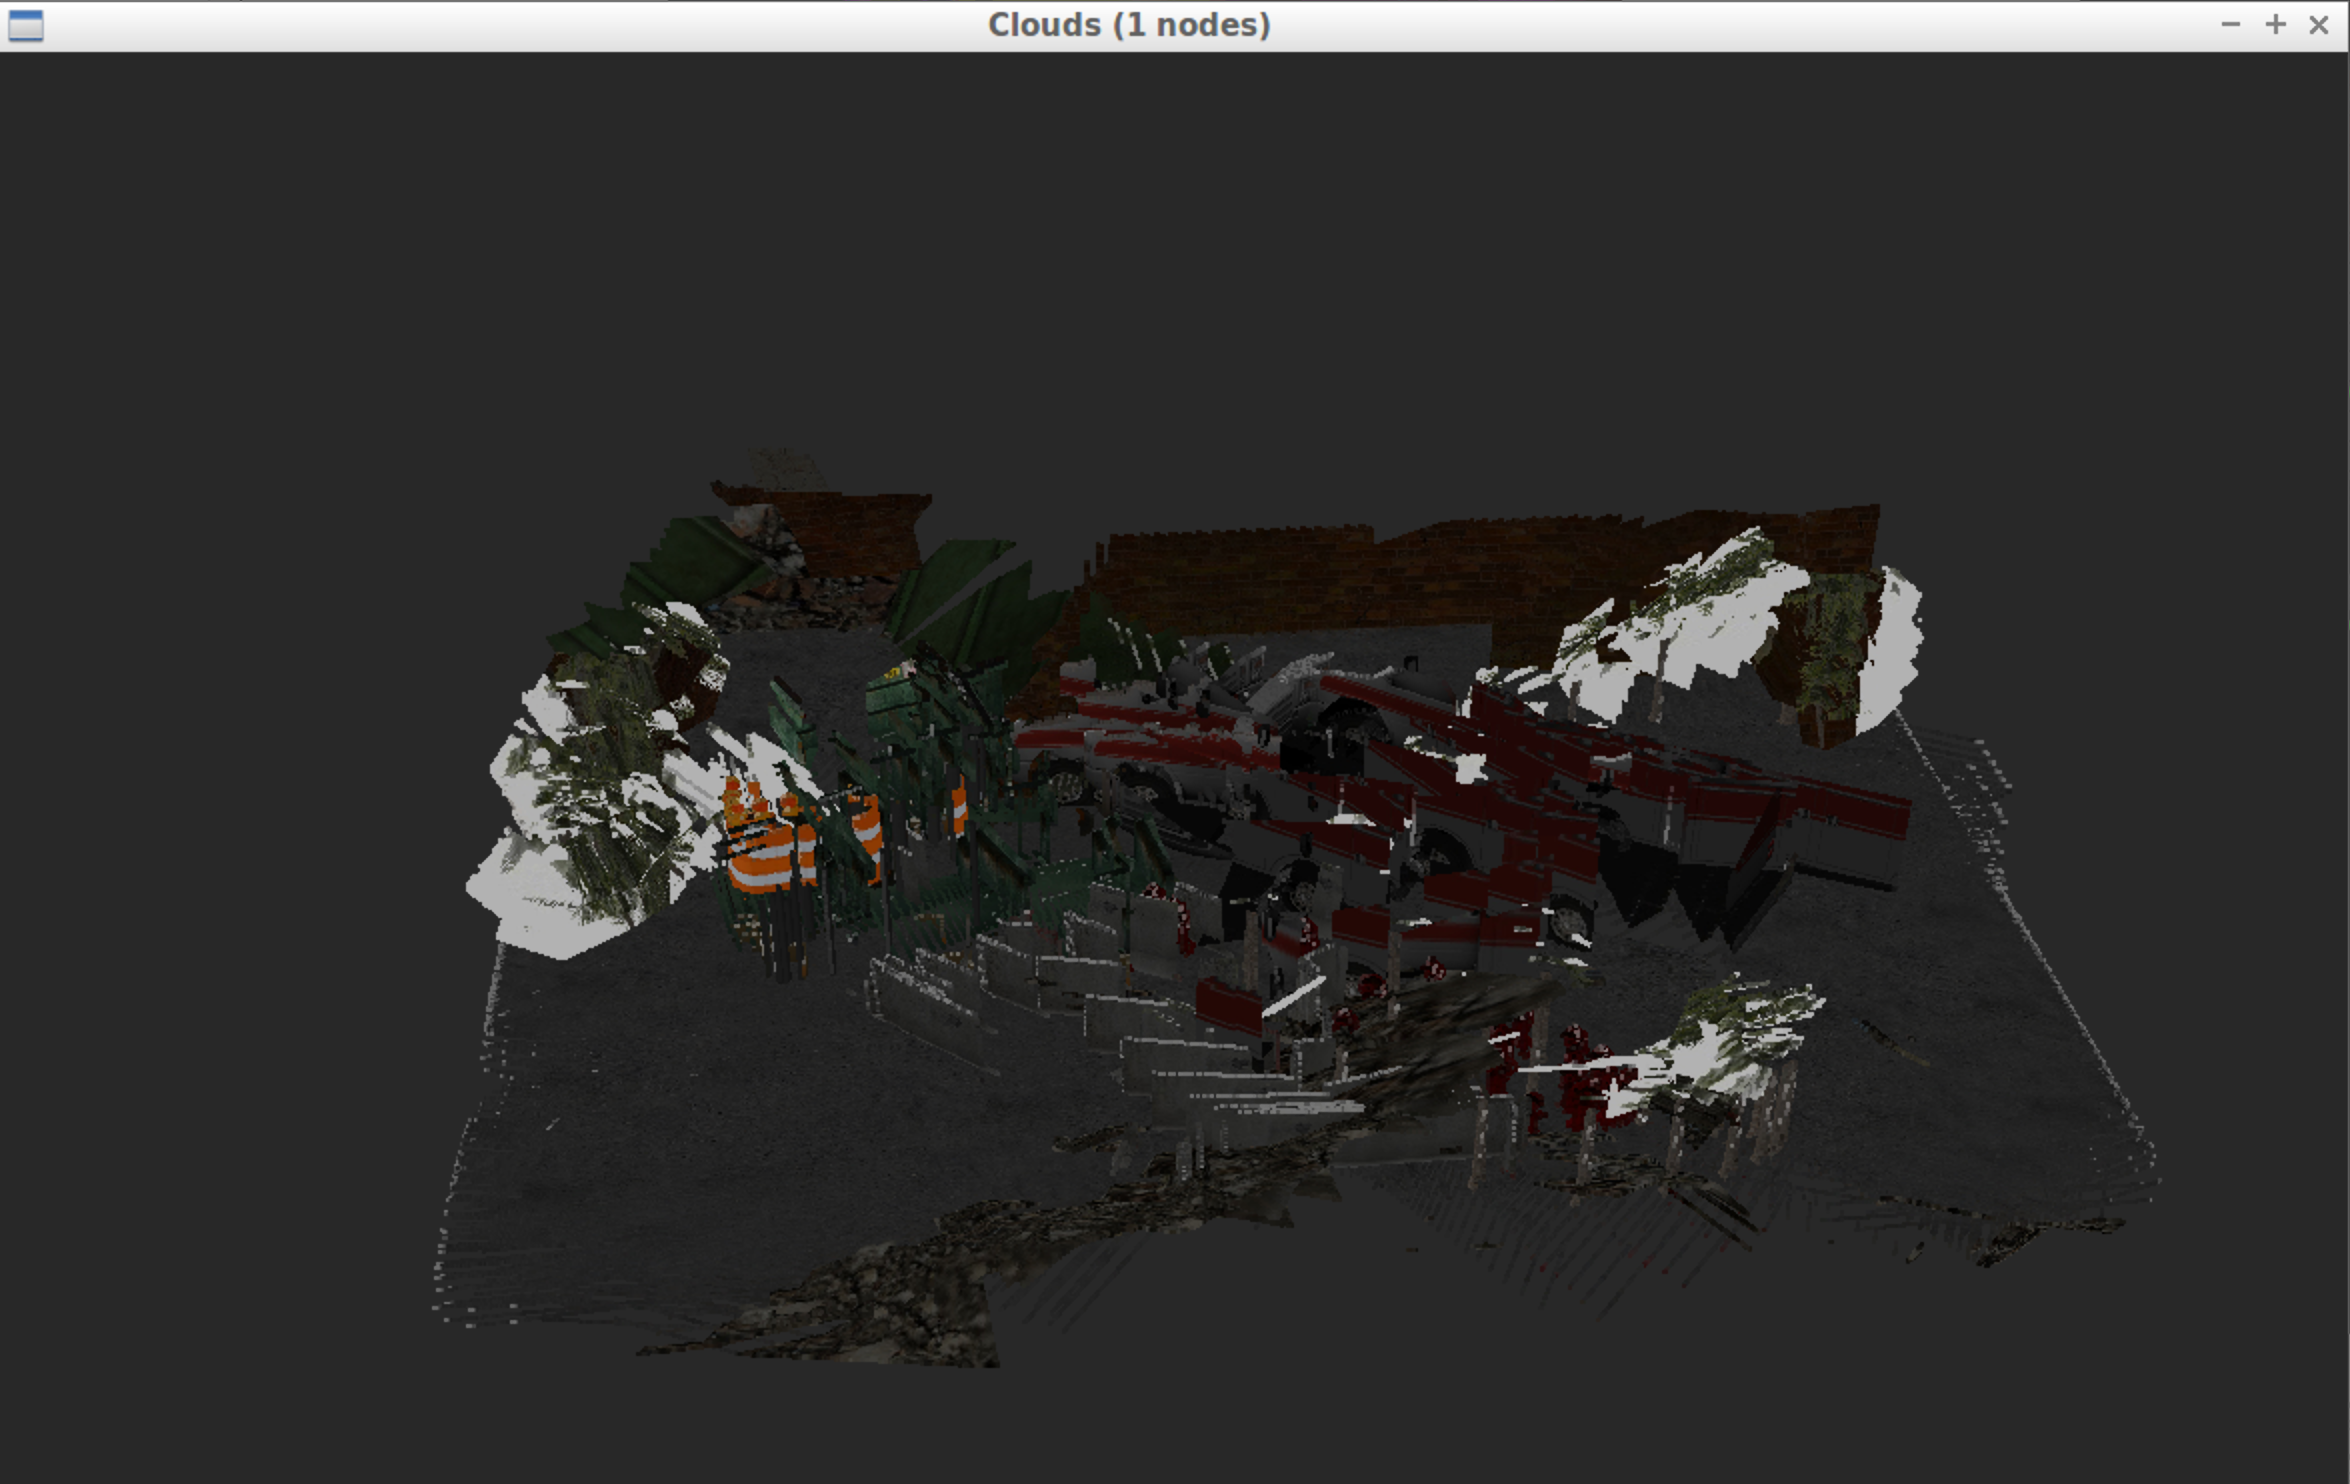
\includegraphics[width=\linewidth]{personal-point-cloud.png}
      \caption{Personal Environment: Point cloud generated through RTAB-Map.}
      \label{fig:network-training}
\end{figure}


\section{Discussion}

Evidently, the algorithm managed to successfully map the kitchen environment but was as successful for the personal environment. The failure to map the personal can be mostly attributed to the lack of sufficient distinguishable features in the environment that the algorithm could rely on. Additionally, due to the size of the personal environment, we navigated the site twice only. This is in order to keep the size of the rtabmap database file within manageable limits.

\section{Conclusion / Future work}

As we saw, the rtabmap algorithm can successfully create a good representation of a survey site, given the site has good amount of structure.

For future, we would investigate that fine tuning some of the parameters available in the ROS RTAB-Map package help to successfully map the constructed personal environment.

Another thing to configure and run the system on hardware that an RGB-D camera and use it to create a 3D mapping of single object or a whole environment such my personal room.

Also, we would like to test the algorithm performance on creating a 3D representation of a living object.

\bibliography{bib}
\bibliographystyle{ieeetr}

\end{document}